The figure~\ref{fig:latency-vs-max-deg} shows how the latency of message delivery per communication radius changes with an increase in the maximum constrained node degree.
The different communication radii are shown as distinct curves on the plot, and shows as expected a trend towards a lower latency with a lower communication radius.
A lower communication radius in turn creates fewer messages, as there are generally fewer links and peers to propagate messages to, which exhibits less strain on the message buffers of the individual hosts.
An important insight that I derive from this plot is that increasing the maximum node degree beyond a certain point does not significantly improve the latency of message delivery, and that increase is echoed in longer communication ranges: in other words, the longer the communication range, the less effect an increase in maximum node degree has on the latency of message delivery.
Surprisingly, higher communication ranges exhibit a positive effect on latency with an increase in maximum node degree, as especially visible in the 100m communication range.

\begin{figure}[htbp]
    \centering
    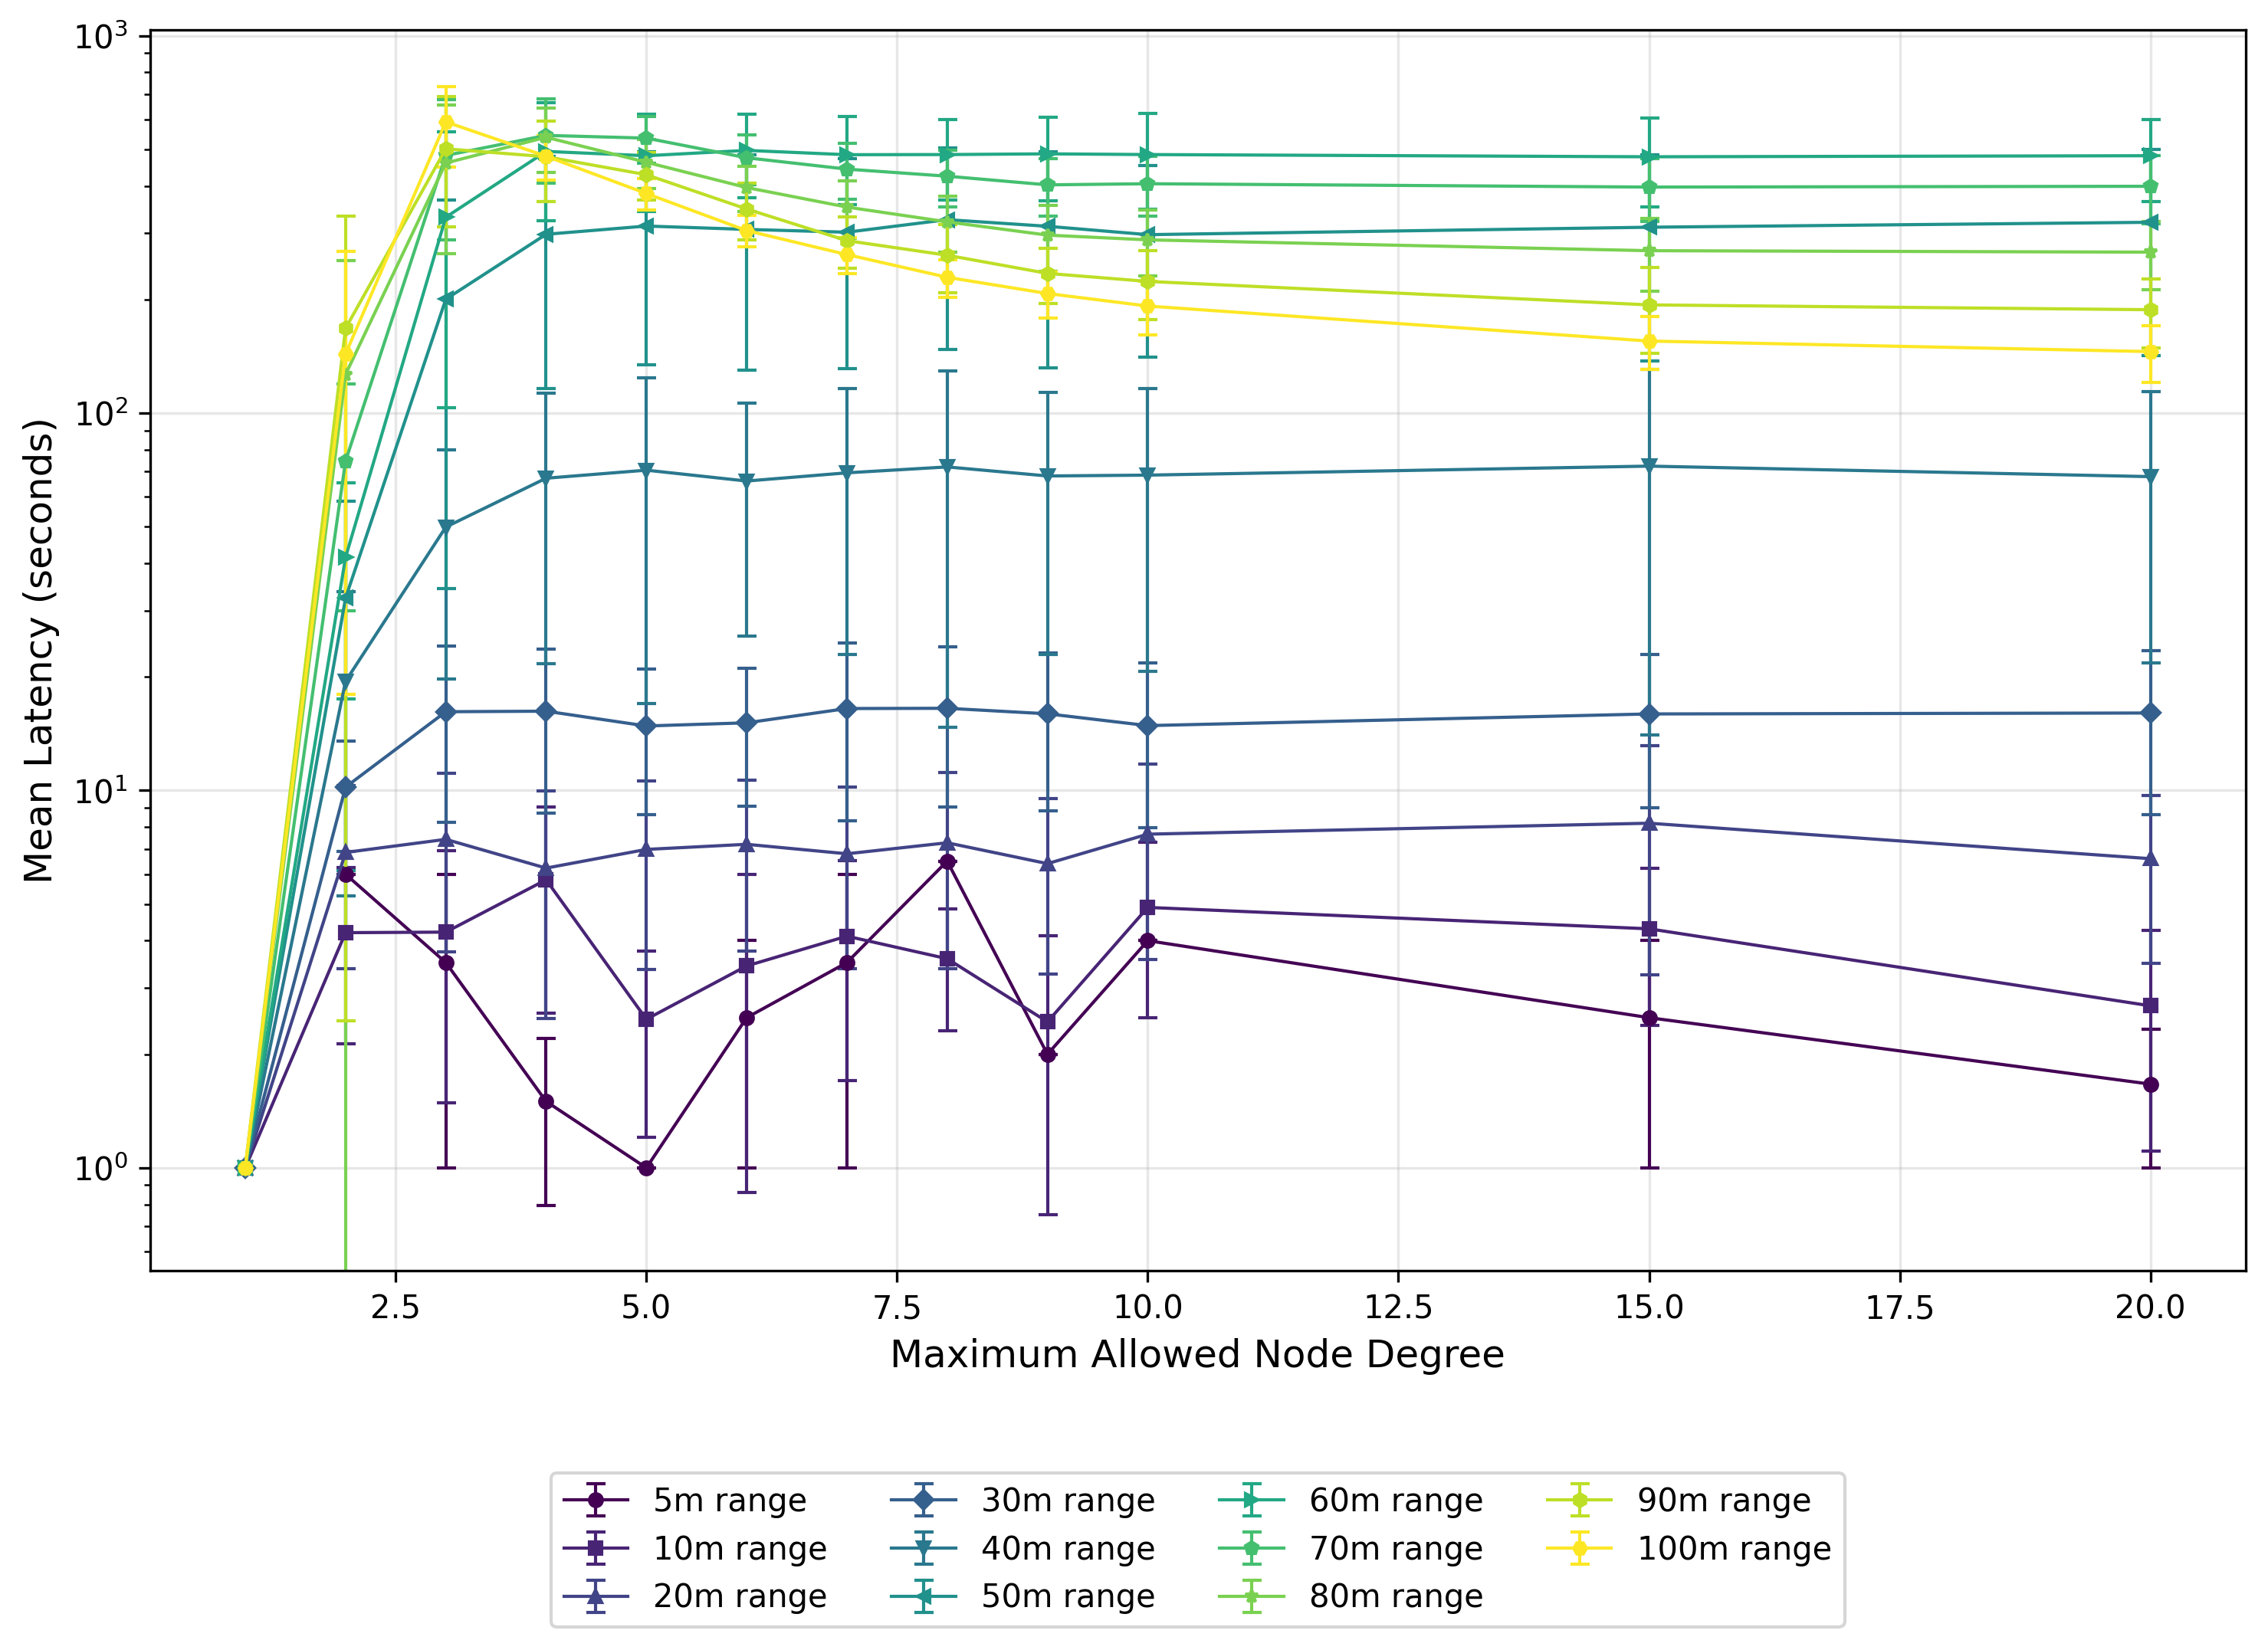
\includegraphics[width=0.5\textwidth]{figures/latency_vs_max_degree_inter_all_dist.png}
    \caption{Latency vs. max node degree - inter-cluster communication}
\label{fig:latency-vs-max-deg}
\end{figure}

\begin{figure}[htbp]
    \centering
    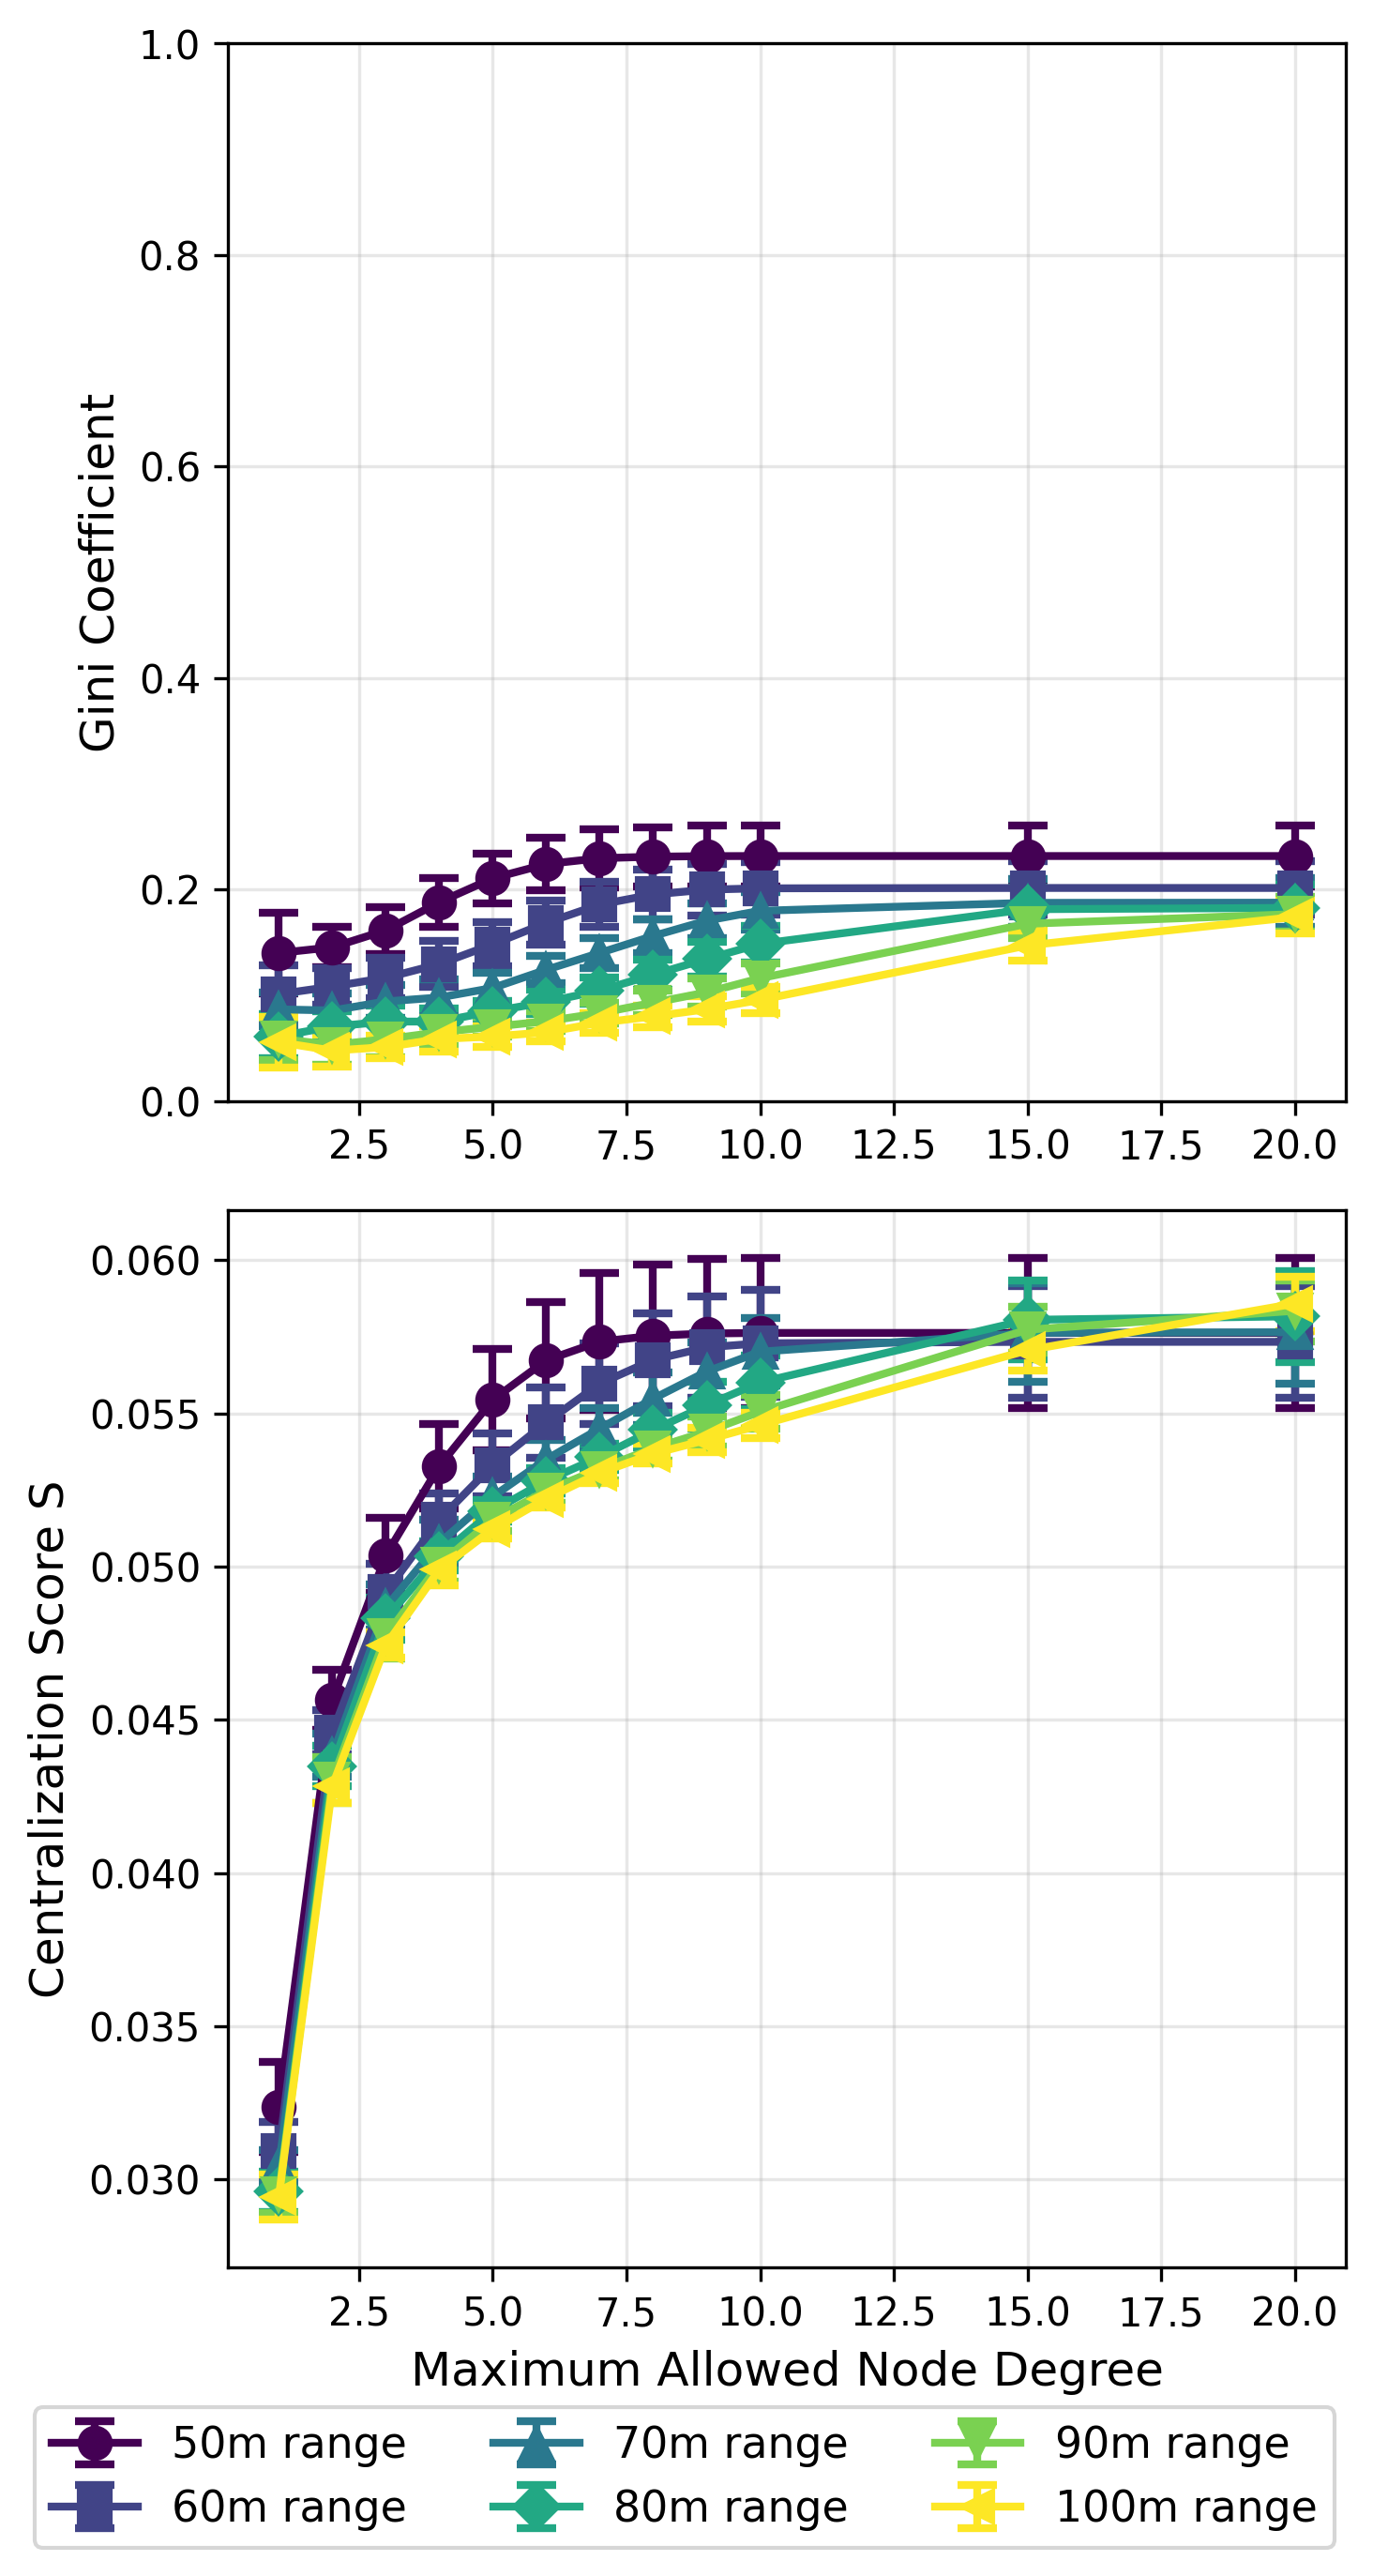
\includegraphics[width=0.5\textwidth]{figures/centralization_metrics_vs_max_degree_inter_high_dist.png}
    \caption{Centralization vs. max node degree - inter-cluster communication}
\label{fig:centralization-vs-max-deg}
\end{figure}

Figure~\ref{fig:centralization-vs-max-deg} shows how the different centralization metrics introduced in section~\ref{sec:state} correlate with an increase in the maximum constrained node degree.
An extended version of this plot, comparing the aforementioned centralization metrics to the L0 norm also in the intra-cluster communication mode, can be found in the appendix, figure~\ref{fig:centralization-vs-max-deg-high}.

Due to the inherent variance in the BLE protocol and high interference demonstrated on wireless channels in the urban settings we used to conduct the empirical time constraints, and some RSSI experiments must be repeated, as evident from figures~\ref{fig:rssi-time},\ref{fig:rssi-pdf}: the 80, 90, and 110 meter plots are jittery: some of which due to having an abnornally low received packet count, which indicates the experiment should be repeated in future work.
The RSSI values we have provided for the ranges that are complete and stable, are mostly sufficient to derive the necessary path loss parameters for the simulation, as they exhibit the expected power-law distribution and are mostly consistent.
% Figure \ref{fig:latency-percentiles} interestingly shows that latency increases with distance, which confirms the path-loss model, but exhibits an unexpected result: we expected the 120m radius simulation result to have the highest latency on average, as it created the most messages and suffers the most from the epidemic routing's flooding of messages, but it was dominated by 50-70m ranges, perhaps due to the missing RSSI values at those distances.
% The centralization metrics plot (Figure \ref{fig:centralization-metrics}) summarizes the simulation results, and proves that L0 loss is indeed not enough to characterise centralization score: it has 1.0 for most values.
% The Gini index and the Centralization score S plots show a positive relation: as the Gini index increases, the S score increases as well, but the curves that dominate the graph are the not the same: the Gini index is dominated by the 40m range, while the S score is dominated by the 120m range.